\subsection{Charakterisierung des Pr:YLF-Kristalls}

\subsubsection{Absorptionsspektrum}

Zur Bestimmung des Absorptionsspektrums des Pr:YLF-Kristalls wurde mit dem USB-Spektrometer ein
Referenzspektrum aufgezeichnet (Tageslicht vom Himmel), dann das Transmissionsspektrum des Kristalls
mit dem gleichen Licht aufgezeichnet und (vom Spektrometer) das Absorptionsspektrum als Differenz
berechnet.
Abb.~\ref{img:AbsSpec} zeigt das berechnete Spektrum.
Die Lage der Absorptionsmaxima ist eingezeichnet und in Tab.~ \ref{tab:AbsSpec} aufgeführt.

Die Zuordnung einiger Linien des Absorptionsspektrums ist mit Hilfe von spektroskopischen Daten
(Tab.~\ref{tab:AbsSpecTh}) möglich.
Die Linien 2-6 können so fünf Übergängen aus dem Grundzustand zugeordnet werden
(Tab.~\ref{tab:AbsSpec}).

\begin{figure}[H]
\begin{center}
  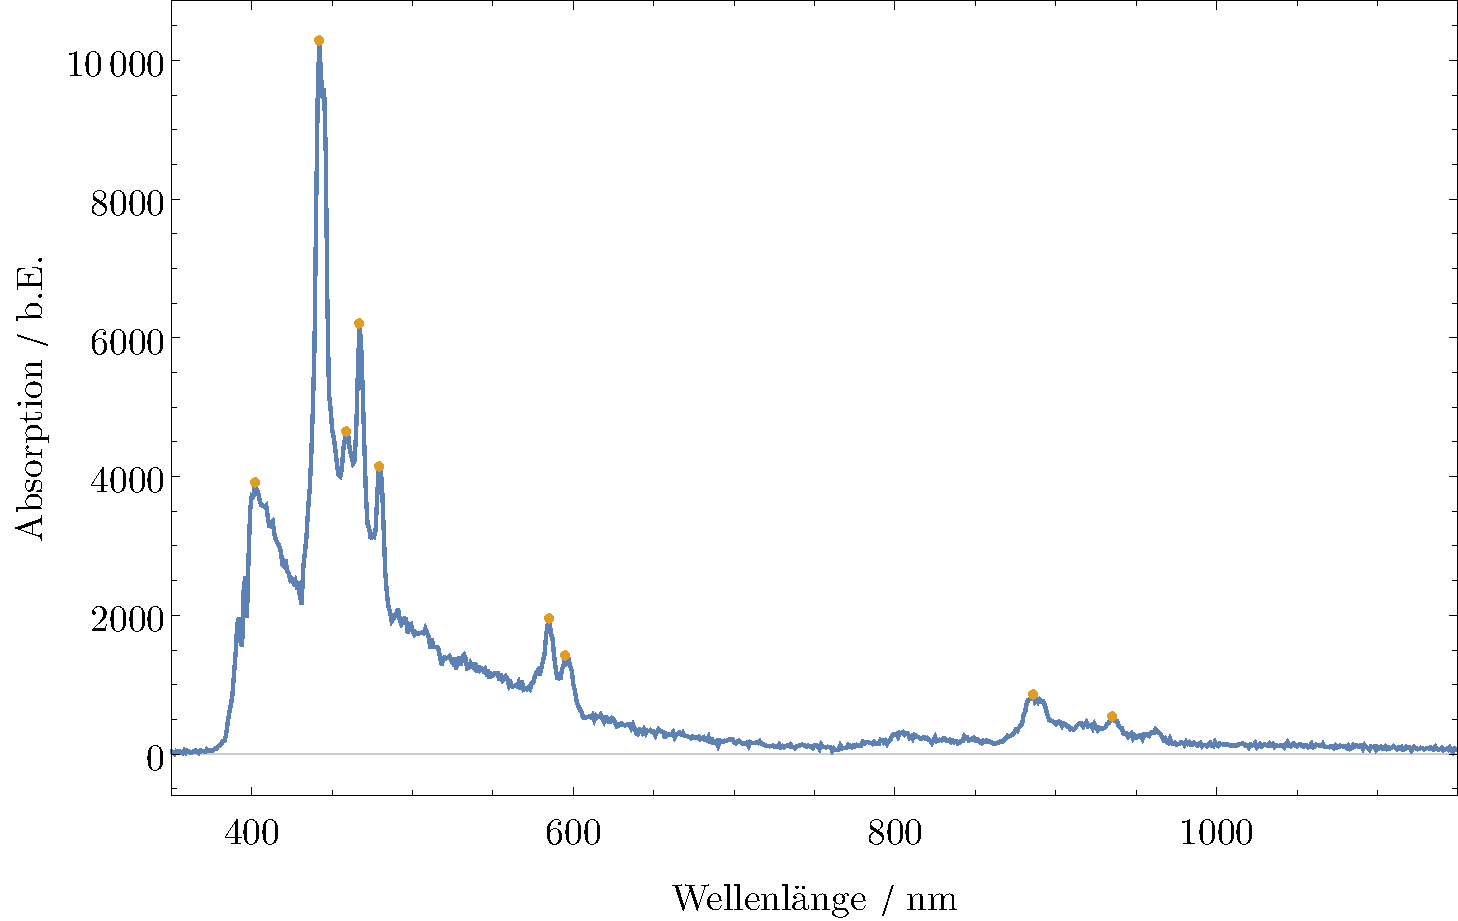
\includegraphics[width=\textwidth]{AbsSpec.pdf}
  \caption{Absorptionsspektrum des Pr:YLF-Kristalls und Position der deutlichen Maxima.}
  \label{img:AbsSpec}
\end{center}
\end{figure}

\begin{table}[htb]
\caption{Positionen und relative Intensitäten der Absorptionsmaxima im Spektrum des
Pr:YLF-Kristalls und Zuweisung der gemessenen Absorptionslinien zu Übergängen in angeregte
Zustände.}
\begin{center}
\begin{tabular}{|c|c|}
\hline
Wellenlänge / nm & Absorption / b.E. \\ \hline
402 & 3918.9 \\ \hline
442 & 10287.3 \\ \hline
459 & 4653.3 \\ \hline
467 & 6203.5 \\ \hline
479 & 4147.4 \\ \hline
585 & 1947.5 \\ \hline
595 & 1420.8 \\ \hline
886 & 850.9 \\ \hline
935 & 535.6 \\ \hline
\end{tabular}
\end{center}
\label{tab:AbsSpec}
\end{table}

\begin{table}[htb]
\caption{Übergänge aus dem Grundzustand $^3$H$_4$ in angeregte Zustände von Pr$^{3+}$
\cite{NIST_ASD}.}
\begin{center}
\begin{tabular}{|c|c|c|}
\hline
Zielniveau & Wellenzahl / cm$^{-1}$ & Wellenlänge / nm \\ \hline
$^3$H$_5$ & 2152.09 & 4646.65 \\ \hline
$^3$H$_6$ & 4389.09 & 2278.38 \\ \hline
$^3$F$_2$ & 4996.61 & 2001.36 \\ \hline
$^3$F$_3$ & 6415.24 & 1558.79 \\ \hline
$^3$F$_4$ & 6854.75 & 1458.84 \\ \hline
$^1$G$_4$ & 9921.24 & 1007.94 \\ \hline
$^1$D$_2$ & 17334.4 & 576.888 \\ \hline
$^3$P$_0$ & 21389.8 & 467.512 \\ \hline
$^3$P$_1$ & 22007.5 & 454.391 \\ \hline
$^3$P$_2$ & 23160.6 & 431.768 \\ \hline
$^1$I$_6$ & 22211.5 & 450.216 \\ \hline
\end{tabular}
\end{center}
\label{tab:AbsSpecTh}
\end{table}

\subsubsection{Emissionsspektrum}

\begin{figure}[H]
\begin{center}
  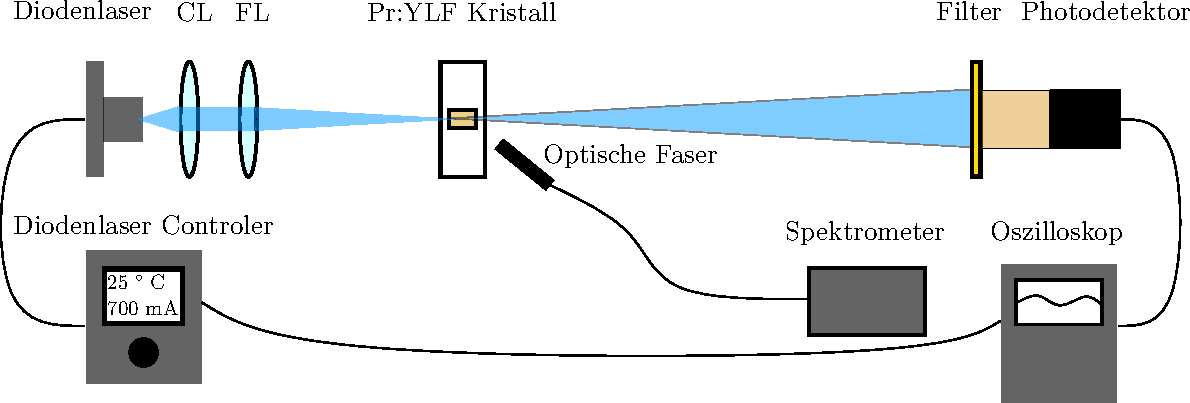
\includegraphics[width=\textwidth]{Aufbau3.pdf}
  \caption{Schematische Darstellung des für die Messung des Emissionsspektrums sowie der
  Lebensdauer des angeregten Zustands verwendeten Aufbaus.
    Der kollimierte Laserstrahl wird mit einer zweiten Linse (FL) mit einer Brennweite von 60\,mm auf
  den Kristall fokussiert, sodass dort eine möglichst große Intensität erzielt wird.
  Eine optische Faser wird so montiert, dass sie auf den Kristall gerichtet ist und an ein
  Spektrometer der Firma Lasertack angeschlossen.
  Das Signal des Spektrometers wird an einem Computer mit dem Programm ''Check Tr\_9\_5''
  aufgenommen.
  Für die Messung der Lebensdauer wird das blaue Licht des Pumplasers über einen GG495 Filter
  geblockt und nur das vom Kristall emittierte Licht transmittiert.
  Das Fluoreszenzlicht des Kristalls wird dahinter mit einem Photodetektor gemessen und
  über eine Widerstandsbox auf einem Oszilloskop angezeigt.
  Das Oszilloskop ist zum Triggern zusätzlich mit dem Diodenlaser Controller verbunden.}
  \label{img:aufbau3}
\end{center}
\end{figure}

Die Messung des Emissionsspektrums erfolgt mit dem Aufbau auf Abb.~\ref{img:aufbau3},
das Messergebnis ist auf Abb.~\ref{img:EmSpec} zu sehen.
In Tab.~\ref{tab:EmSpec} sind die Positionen der Absorptionsspitzen aufgeführt und
es werden einige Linien mit Übergängen von Pr$^{3+}$
identifiziert.

\begin{figure}[H]
\begin{center}
  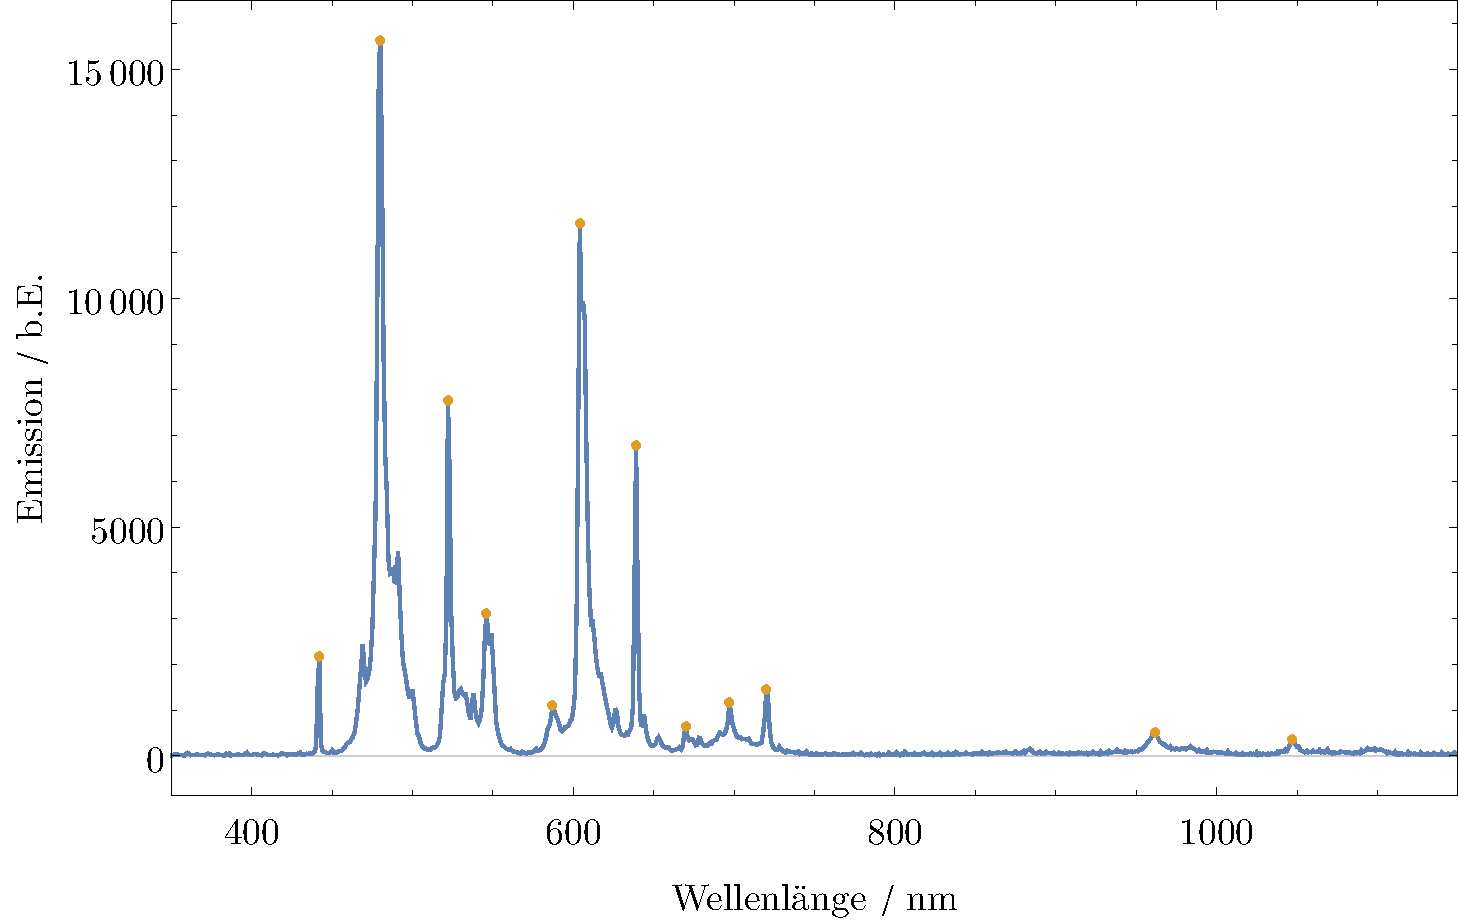
\includegraphics[width=\textwidth]{EmSpec.pdf}
  \caption{Emissionsspektrum des Pr:YLF-Kristalls und Position der deutlichen Maxima.}
  \label{img:EmSpec}
\end{center}
\end{figure}

\begin{table}[htb]
\caption{Positionen und relative Intensitäten der Emissionsmaxima im Spektrum des
Pr:YLF-Kristalls sowie Zuweisung der Linien zu den Übergängen.}
\begin{center}
\begin{tabular}{|c|c|}
\hline
Wellenlänge / nm & Emission / b.E. \\ \hline
442 & 2168.6 \\ \hline
480 & 15633.9 \\ \hline
522 & 7761.3 \\ \hline
546 & 3115.6 \\ \hline
587 & 1099.0 \\ \hline
604 & 11627.5 \\ \hline
639 & 6787.0 \\ \hline
670 & 635.9 \\ \hline
697 & 1162.8 \\ \hline
720 & 1457.7 \\ \hline
962 & 508.6 \\ \hline
1047 & 366.7 \\ \hline
\end{tabular}
\end{center}
\label{tab:EmSpec}
\end{table}


\FloatBarrier


\subsubsection{Messung der Lebensdauer des angeregten Zustands}

\paragraph{Aufbau und Durchführung}

Für diesen Versuchsteil wird der in Abb.~\ref{img:aufbau3} dargestellte Aufbau verwendet.
Der Pumplaser wird hierbei im modulierten Bereich bei 710\,mA betrieben und das Oszilloskop darüber
getriggert. Das Signal des Photodetektors geht über eine Widerstandsbox, welche bei 1\,k$\Omega$
betrieben wird, ebenfalls auf das Oszilloskop.

\paragraph{Auswertung}
Abb.~\ref{img:Lifetime} zeigt die Modulation der Laserspannung während der Messung und das
dazugehörige Fluoreszenzsignal, das von der Photodiode geliefert wird.
Das Photodiodensignal eines einzelnen Abschaltvorgangs ist auf Abb.~\ref{img:LifetimeFit} zu sehen. 
Als Fehler auf die Diodenspannung wird von der Spannungsauflösung des Oszilloskops
(0.2\,mV) ausgegangen und diese - unter Annahme einer Gleichverteilung der Fehler - durch
$2\sqrt{3}$ geteilt.
Der Fit des Signals erfolgt mit einer exponentiellen Abnahme mit der Zeitkonstanten~$\tau$ und dem
Untergrund~$U$. Das Fitergebnis ist auf Tab.~\ref{tab:Fit_lifetime} zu sehen.


\begin{figure}[H]
\begin{center}
  \includegraphics[width=.7\textwidth]{lifetime.png}
  \caption{Modulation des Lasers mit einem Rechtecksignal (gelb) zur Bestimmung der Lebensdauer der
  Fluoreszenz (blau, Messung als Spannungssignal der Photodiode).}
  \label{img:Lifetime}
\end{center}
\end{figure}


\begin{figure}[H]
\begin{center}
  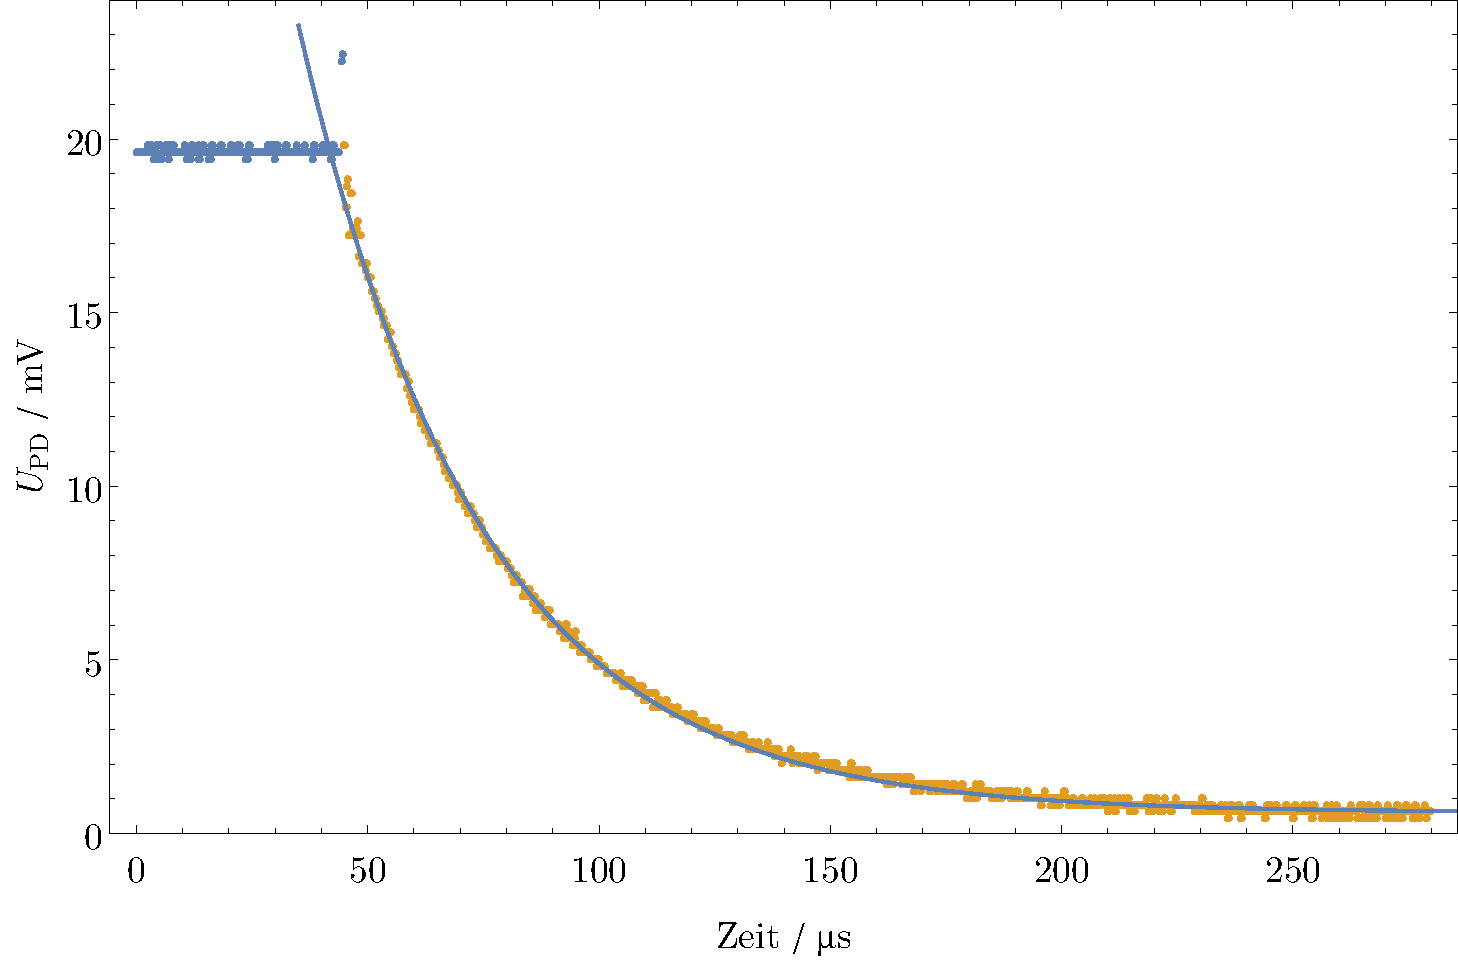
\includegraphics[width=.9\textwidth]{lifetime.pdf}
  \caption{Exponentieller Fit des Spannungssignals der Photodiode $U_{\text{PD}}$ zur Bestimmung der
  Lebenszeit des angeregten Zustands. Der Fitbereich ist gelb markiert, auf die Darstellung der geringen Fehler
  wurde verzichtet.}
  \label{img:LifetimeFit}
\end{center}
\end{figure}

\begin{table}[htb]
\caption{Ergebnisse des Fits der Fluoreszenzlebensdauer mit
$y=A\,\exp(-x/\tau)\,+\,U$.}
\begin{center}
\begin{tabular}{|c|c|}
\hline
$A$ & 55.65\,$\pm$\,0.21\,mV \\ \hline
$\tau$ & 39.01\,$\pm$\,0.10\,\textmu s \\ \hline
$U$ & 0.605\,$\pm$\,0.008\,mV \\ \hline
\textchi$^2$ & 527.875 \\ \hline
\textchi$^2$/\,DoF & 0.450021 \\ \hline
\end{tabular}
\end{center}
\label{tab:Fit_lifetime}
\end{table}


\subsubsection{Messung der absorbierten Leistung}

\paragraph{Aufbau und Durchführung}

\begin{figure}[H]
\begin{center}
  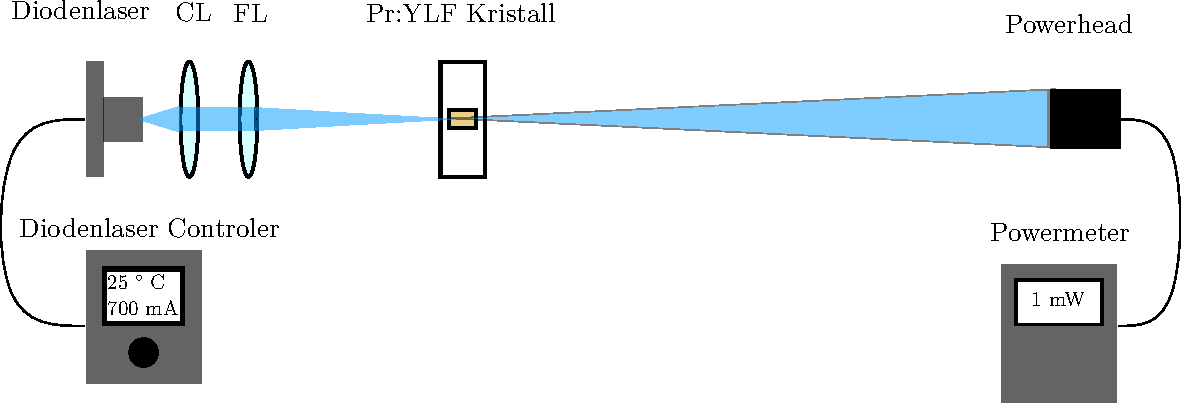
\includegraphics[width=\textwidth]{Aufbau2.pdf}
  \caption{Schematische Darstellung des für die Messung der absorbierten Leistung verwendeten
  Aufbaus. Hierfür entfernen wir den Filter wieder und ersetzten den Photodetektor mit dem
  Powerhead, welcher an das Powermeter angeschlossen wird.}
  \label{img:aufbau2}
\end{center}
\end{figure}

Wir verwenden hier den in Abb.~\ref{img:aufbau2} dargestellten Aufbau. Für 400\,mA, 600\,mA und
800\,mA wurden jeweils bei 25\grad und 35\grad die Leistungen mit und ohne Kristall im Strahlengang
gemessen.



\paragraph{Auswertung}
Die so gemessenen Leistungswerte sind auf Tab.~\ref{tab:Absorption} zu sehen.
Die Differenz der Messwerte $P_\text{ohne}$ und $P_\text{mit}$ ist die im Kristall
absorbierte Leistung $P_\text{abs}$.
Durch Division durch $P_\text{ohne}$ wird die relative Absorption berechnet.

\begin{table}[htb]
\caption{Leistung am Leistungsmesskopf ohne Kristall im Strahlengang ($P_\text{ohne}$),
mit Kristall ($P_\text{mit}$), absorbierte Leistung ($P_\text{abs}$) und relative Absorption
$P_\text{abs}/P_\text{ohne}$ in Abhängigkeit von Lasertemperatur $T$ und Laserstrom $I$.}
\begin{center}
\begin{tabular}{|c|c|c|c|c|c|}
\hline
T / \grad & I / mA & $P_\text{mit}$ / mW & $P_\text{ohne}$ / mW & $P_\text{abs}$ / mW & Absorption / \% \\ \hline
25 & 400 & 114 & 427 & 313 & 73.3 \\ \hline
25 & 600 & 149 & 737 & 588 & 79.8 \\ \hline
25 & 800 & 87.4 & 532 & 444.6 & 83.6 \\ \hline
35 & 400 & 77.1 & 408 & 330.9 & 81.1 \\ \hline
35 & 600 & 105 & 718 & 613 & 85.4 \\ \hline
35 & 800 & 30.6 & 522 & 491.4 & 94.1 \\ \hline
\end{tabular}
\end{center}
\label{tab:Absorption}
\end{table}
